\chapter{When transitions are uniform POIBMDPs are fully observable}
In this section we show that decision tree induction for classification problems can be formulated as solving POIBMDPs.
Indeed, a supervised classification problem (cite) can be formulated as an MDP where actions are class labels and states are training data.
The reward at every step is 1 if the correct label was predicted and 0 otherwise.
In this MDP, the transitions are independent of the actions: the next state is given by uniformly sampling a new training datum. 
This implies that the resulting POIBMDP is actually \textit{fully} observable and that traditional RL algorithms should perform well.

\begin{definition}[Classification Markov Decision Process]
    Given a set of $N$ examples denoted $\mathcal{E} = {\{(x_i, y_i)\}}_{i=1}^N$ where each datum $x_i$ is described by a set of $p$ features and $y_i \in \mathbb{Z}^m$ is the label associated with $x_i$, a Classification Markov Decision Process is an MDP (cite) $\langle S, A, R, T, T_0 \rangle$ where:
    \begin{itemize}
        \item the state space is $S={\{x_i\}}_{i=1}^N$, the set of data features
        \item the action space is $A=\mathbb{Z}^m$, the set of unique labels
        \item the reward function is $R:S\times A \rightarrow \{0, 1\}$ with $R(s=x_i, a) = 1_{a=y_i}$
        \item the transition function is $T:S\times A \rightarrow \Delta S$ with $T(s, a, s') = \frac{1}{N} \quad \forall s, a, s'$
        \item the initial distribution is $T_0(s_0 = s) = \frac{1}{N}$
    \end{itemize}
\end{definition}

\begin{figure}[h]
    \centering
    \begin{tikzpicture}[
        decision/.style={circle, draw, thick, fill=blue!20, text width=2.5em, text centered, minimum height=2.5em, font=\small},
        leaf/.style={rectangle, draw, thick, fill=green!20, text width=2em, text centered, rounded corners, minimum height=2em, font=\small},
        edge_label/.style={font=\footnotesize, midway}
    ]
        % Tree 4: if x <= 0.5 move right else move left
        \node[decision] (tree4_root) at (8,2) {$x \leq 1$};
        \node[rectangle, draw, thick, fill=green!40, text width=2em, text centered, rounded corners, minimum height=2em, font=\small] (tree4_right) at (7,0) {};
        \node[rectangle, draw, thick, fill=red!40, text width=2em, text centered, rounded corners, minimum height=2em, font=\small] (tree4_left) at (9,0);
        \draw[->] (tree4_root) -- (tree4_right) node[edge_label, above left] {True};
        \draw[->] (tree4_root) -- (tree4_left) node[edge_label, above right] {False};
        \tikzstyle{grid}=[draw, thick, fill=gray!10]
        
        % Draw grid
        \draw[fill=green!40] (0, 0) rectangle (1,2);
        \draw[fill=red!40] (1, 0) rectangle (2,2);

        \draw[grid] (0,0) grid (2,2);
        
        % Add axes
        \draw[thick, ->] (0,0) -- (2.5,0) node[right] {$x$};
        \draw[thick, ->] (0,0) -- (0,2.5) node[above] {$y$};
        
        % Add tick marks and labels
        \foreach \x in {0,1,2} {
            \draw[thick] (\x,0) -- (\x,-0.1) node[below] {$\x$};
        }
        \foreach \y in {0,1,2} {
            \draw[thick] (0,\y) -- (-0.1,\y) node[left] {$\y$};
        }

        \node at (0.5,0.5) {$s_0$};
        \node at (1.5,0.5) {$s_g$};
        \node at (1.5,1.5) {$s_2$};
        \node at (0.5,1.5) {$s_1$};

    \end{tikzpicture}
    \caption{Classification MDP optimal actions. In this Classification MDP, there are four data to assign either a green or red label.
    On the right, there is the unique optimal depth-1 tree for this particular Classification MDP. This depth-1 tree also maximizes the accuracy on the corresponding classification tasks.}
    \end{figure}

It is easy to see that policies that maximize the expected discounted cumulative reward objective (cite) are classifiers that maximize the prediction accuracy because $\sum_{i=1}^N 1_{\pi(x_i)=y_i} = \sum_{i=1}^N R(x_i, \pi(x_i))$.
We defer the formal proof in the next part of the manuscript in which we extensively study supervised learning problems.
Learning a classifier with a reward signal can also be done with contextual bandits (cite).

To learn a decision tree \textit{classifier}, we use the POIBMDP formalism and show, in the particular case where the base MDP is a Classification MDP (cite), that associated POIBMDPs are in fact MDPs with stochastic transitions. 
\begin{definition}[Classification POIBMDP]
    Given a Classification MDP (cite) $\langle {\{x_i\}}_{i=1}^N, \mathbb{Z}^m, R, T, T_0 \rangle$, and an associated POIBMDP (cite) $\langle S, O, A, A_{info}, R, \zeta, T_{info}, T, T_0\rangle$, a Classification POIBMDP is an MDP:
    \begin{align*}
        \langle \overbrace{O}^{\text{State space}}, \underbrace{\mathbb{Z}^m, A_{info}}_{\text{Action space}}, \overbrace{R, \zeta}^{\text{Reward function}}, \underbrace{\mathcal{P}, \mathcal{P}_0}_{\text{Transition kernels}} \rangle
    \end{align*}
    \begin{itemize}
        \item $O$ is the set of possible observations in $[L_1, U_1] \times \dots \times [L_d, U_d] \times [L_1, U_1] \ times \dots \times [L_d, U_d] $ where $L_j$ is the minimum value of feature $j$ over all data $x_i$ and $U_j$ the maximum
        \item $\mathbb{Z}^m \cup A_{info}$ is action space: actions can be label assignments in $\mathbb{Z}^m$ or bounds refinement in $A_{info}$
        \item The reward for assigning label $a\in \mathbb{Z}^m$ when observing some observation $o=(L'_1, U'_1, \dots, L'_d, U'_d)$ is the proportion of training data satistifying the bounds and having label $a$: $R(o, a) = \frac{|\{x_i: L'_j \leq x_{ij} \leq U'_j \forall i,j \} \cap \{x_i: y_i = a \forall i \}|}{|\{x_i: L'_j \leq x_{ij} \leq U'_j \forall i,j \}|}$. 
        The reward for taking an information gathering action that refines bounds is $\zeta$
        \item The transition kernel is $\mathcal{P}:O \times (\mathbb{Z}^m \cup A_{info}) \rightarrow \Delta O$ where:
        \begin{itemize}
            \item For $a \in \mathbb{Z}^m$: $\mathcal{P}(o, a, (L_1, U_1, \dots, L_d, U_d)) = 1$ (reset to full bounds)
            \item For $a = (k, v) \in A_{info}$: from $o=(L'_1, U'_1, \dots, L'_d, U'_d)$, the MDP will transit to $o_{left} = (L'_1, U'_1, \dots, L_k, v, dots, L'_d, U'_d)$ (resp. $o_{right} = (L'_1, U'_1, \dots, U'_k, v, dots, L'_d, U'_d)$) with probability $\frac{|\{x_i: L'_j \leq x_{ij} \leq U'_j \forall j \land x_{ik} \leq v\}|}{|\{x_i: L'_j \leq x_{ij} \leq U'_j \forall j\}|}$ (resp. $\frac{|\{x_i: L'_j \leq x_{ij} \leq U'_j \forall j \land x_{ik} > v\}|}{|\{x_i: L'_j \leq x_{ij} \leq U'_j \forall j\}|}$)
        \end{itemize}
    \end{itemize}
\end{definition}

Now we can learn a decision tree \textit{classifier} for a supervised learning task as follows. 
Given a set of examples and lables, we can formulate the associated Classification MDP (cite). 
Then we can provide some information gathering actions and a reward $\zeta$ for those to define a Classification POIBMDP (cite).
Finally, we can learn a deterministic policy $\pi : O \rightarrow A\cup A_{info}$ to obtain a decision tree classifier. 
Since we have shown that Classification POIBMDPs are MDPs, we that RL baselines should perform well to solve Classification POIBMDPs. 
We expect that, compared to general POIBMDPs studied in the previous chapter where some information was hidden to the agent, RL baselines will consistently learn the optimal decision tree classifiers.

\section{How well can RL baselines learn in Classification POIBMDPs?}
Similarly to the previous chapter, we are interested in a very simple Classification POIBMDP that corresponds to building a tree for the supervised problem:

\begin{align*}
    \mathcal{X} &= \{(0.5, 0.5), (0.5, 1.5), (1.5, 1.5), (1.5, 0.5)\}\\
    y &= \{0, 0, 1, 1\} 
\end{align*}

We illustrate the associated Classification MDP in Figure (cite). 
We construct Classification POIBMDPs with $\gamma=0.99$, 200 values of $\zeta \in [0,1]$ and IGAs $x\leq 1$ and $y\leq 1$.
Since Classification POIBMDPs are MDPs, we do not need to analyze asymmetric and JSJ (cite) baselines.

\begin{figure}
    \centering
    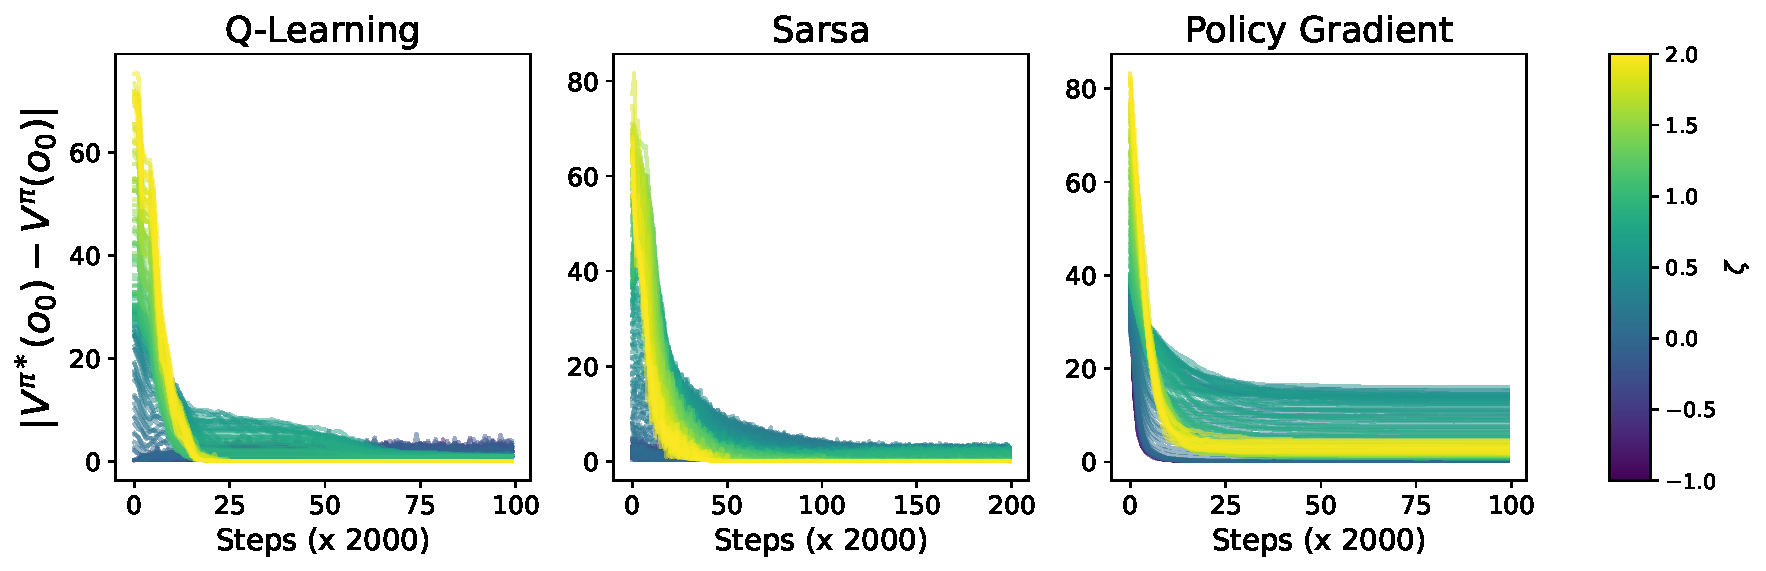
\includegraphics[width=1\textwidth]{images/images_part1/learning_curves_classif.pdf}
    \caption{}\label{fig:rl-classif-poibmdp}
\end{figure}

\begin{figure}
    \centering
    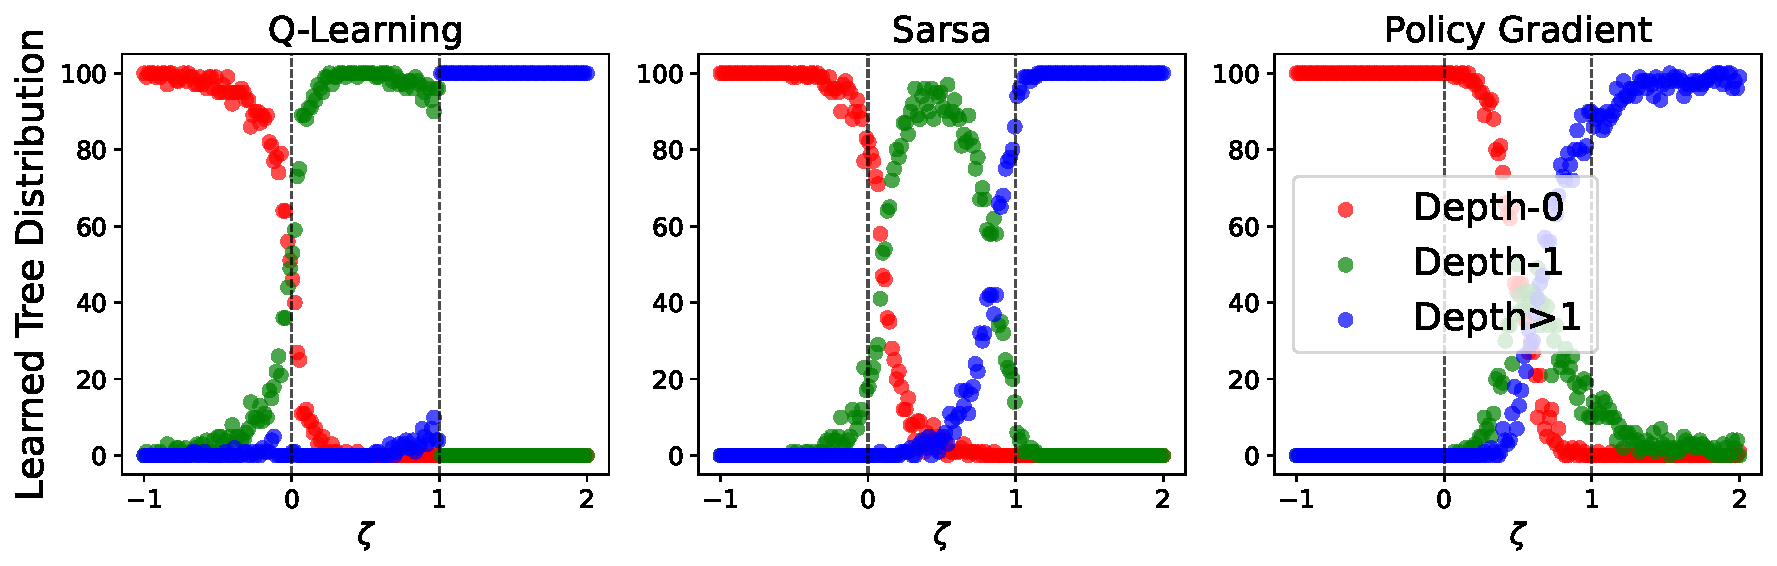
\includegraphics[width=1\textwidth]{images/images_part1/tree_distributions_classif.pdf}
    \caption{}\label{fig:tree-distrib-classif-poibmdp}
\end{figure}

Fortunately this time, compared to general POIBMDPs, RL can be used to retrieve optimal policies in Classification POIBMDPs equivalent to decision tree classifiers.
We observe on Figure (cite) that both Q-learning and Sarsa consistently minimize the sub-optimality gap. 
Hence they are able to retrieve the optimal detph-1 decision tree classifier from Figure (cite).

In this part of the manuscript, we have highlighted the challenges of reinforcement learning of decision tree policies for MDPs.
We showed that this task was particularly challenging, even when an optimal decision tree policy exists.
We saw that RL algorithms are unable to find such optimal trees, even for very simple problems such as a $2\times 2$ grid world.
However, we also showed that for some MDPs, such as ones that encode a supervised learning task, RL algorithms could retrieve optimal decision tree classifiers.
This was shown only on a very simple classification task with four data and two classes.
Furthermore, good candidate nodes--information gathering actions--were provided to the learning algorithms.

Now remains the question of scalability and competitiveness of such approaches to supervised learning for which strong baselines have existed for decades.
In the next part of this thesis; we present a new decision tree induction that relies on solving MDPs exactly and choosing information gathering actions adaptively.



